\documentclass{article}
\usepackage[paperwidth=3.1in,paperheight=4.1in,margin=0in]{geometry}
\usepackage{mathptmx}%{times}
\usepackage{graphicx}
\usepackage{siunitx}
\usepackage[absolute,overlay]{textpos}
\usepackage{color}

\setlength{\parindent}{0pt}
\begin{document}
\TPMargin{3pt}
\textblockcolour{white}
\begin{textblock}{1.5}(13.3,0.2)
\normalsize
\centering
(a)
\end{textblock}
\begin{textblock}{5.5}(9.3,0.9)
\normalsize
$\ell_2 = \num{5.86e-8}$
\end{textblock}
\begin{textblock}{1.5}(13.3,7.4)
\normalsize
\centering
(b)
\end{textblock}
\begin{textblock}{5.5}(9.3,8.2)
\normalsize
$\ell_2 = \num{5.94e-6}$
\end{textblock}
\centering
\includegraphics[width=3in]{../thermalAdvection-btf-250m-50dz/18000/tracerDiffMountain.pdf} \\
\vspace*{0.1in}
\includegraphics[width=3in]{../thermalAdvection-cutCell-250m-50dz/18000/tracerDiffMountain.pdf} \\
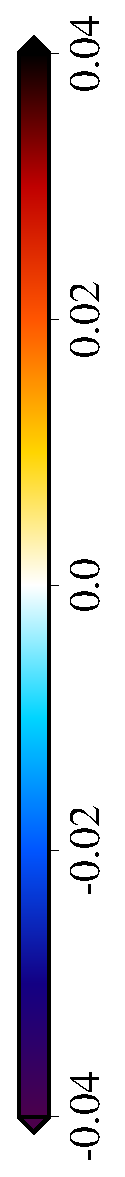
\includegraphics[height=3in,angle=270]{tracerDiffMountain_T_diff.eps}
\end{document}
